% !TEX root = knottedMain.tex
\documentclass[varwidth=\maxdimen]{standalone}

\usepackage{mathtools,amssymb,mathrsfs,dutchcal,upgreek,faktor,accents,etoolbox,multicol}
\usepackage[dvipsnames]{xcolor}
\definecolor{mygreen}{RGB}{	8,156,79 }
\usepackage{tikz,tikz-cd}
\usetikzlibrary{patterns,knots,arrows.meta,decorations.markings}
\tikzset{>={Straight Barb[scale=0.85]}}
\tikzcdset{
  cells={font=\everymath\expandafter{\the\everymath\displaystyle}},
  arrow style=tikz,
  diagrams={>={Straight Barb[scale=0.85]}},
  every label/.append style = {font = \small}
}


\begin{document}
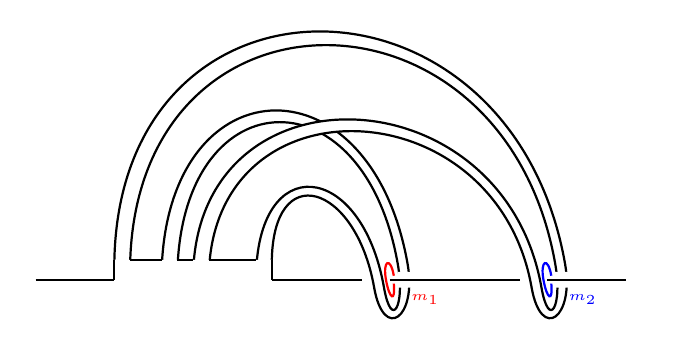
\begin{tikzpicture}[scale=0.5,even odd rule,line width=0.2mm]
    \clip (-1.2,-1.2) rectangle (14.5,6.4);
    \draw[thick]
    %unutarnja druga
                        (4.6,0)
                        to[out=90,in=100, distance=3.3cm] (8-.15,-0.2)
                        to[out=-80,in=-80, distance=1.1cm] (8+.2,0.4)
                        to[out=100,in=90, distance=5.1cm]
                        (2.6,0)
    %spoljna druga
                        (2.2,0)
                        to[out=90,in=100, distance=5.5cm] (8+.45,0.4)
                        to[out=-80,in=-80, distance=1.4cm] (8-.4,-0.2)
                        to[out=100,in=90, distance=2.7cm] (5,0.4) ;
    \fill[white,draw=black,thick]
    %unutarnja prva
                        (3,0)
                        to[out=90,in=100, distance=5.6cm] (12-.15,-0.2)
                        to[out=-80,in=-80, distance=1.1cm] (12+.2,0.4)
                        to[out=100,in=90, distance=7.6cm]
                        (1.4,0.2)
    %spoljna prva
                    -- (1,0.3) to[out=90,in=100, distance=8cm] (12+.45,0.4)
                        to[out=-80,in=-80, distance=1.4cm] (12-.4,-0.2)
                        to[out=100,in=90, distance=5.2cm]
                        (3.4,0) -- cycle ;
    % for crossings
    \fill[white]
            (1,-0.5) rectangle (5,0.5)
            (8.2,-0.2) rectangle (8.6,0.2)
            (12.2,-0.2) rectangle (12.6,0.2) ;
    % missing parts
    \draw[thick]
            (1,0) -- (1,0.5) (5,0)-- (5,0.5)
            (1.4,0.5) -- (2.2,0.5) (2.6,0.5) -- (3,0.5) (3.4,0.5)--(4.6,0.5) ;
    \draw[thick]
            (-1,0) -- (1,0) (5,0) -- (7.3,0) (8,0)  -- (11.3,0)   (12,0) -- (14,0) ;

    \draw[red,thick] 
        (8.1,0.1) to[out=100,in=100, distance=0.5cm] (7.9,0) to[out=-80,in=-85, distance=0.5cm] (8.1,-0.1)
        (8.9,-0.5) node{\tiny$m_1$} ;
    \draw[blue,thick] 
        (12.1,0.1) to[out=100,in=100, distance=0.5cm] (11.9,0) to[out=-80,in=-85, distance=0.5cm] (12.1,-0.1) 
        (12.9,-0.5) node{\tiny$m_2$} ;

\end{tikzpicture}
\qquad
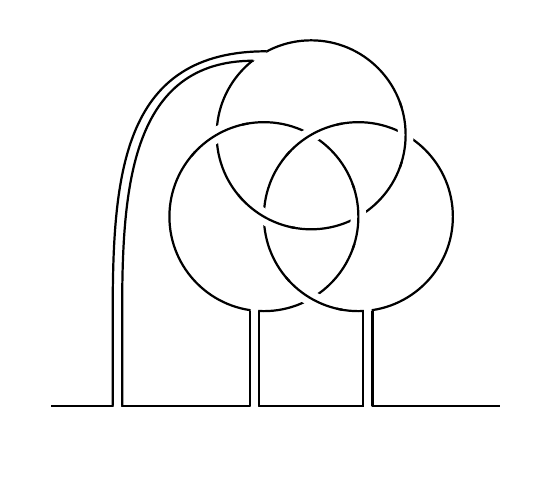
\begin{tikzpicture}[scale=0.6]
\clip (-6,-5) rectangle (4.2,4);

\draw[thick] (-5.5,-4) -- (4,-4);

\begin{knot}[
%  draft mode=crossings,
  flip crossing/.list={3,4},
  clip width=7
]
    \strand[black,thick] (1,0) circle[radius=2cm];
    \strand[black,thick] (-1,0) circle[radius=2cm];
    \strand[,thick] (0,{sqrt(3)}) circle[radius=2cm];
\end{knot}

\fill[white]    (-1.28,-1.9) rectangle (-1.12,-2.1) 
                (-1.28,-4.1) rectangle (-1.12,-3.9);
\fill[white]    (1.28,-1.9) rectangle (1.12,-2.1)
                (1.28,-4.1) rectangle (1.12,-3.9);
\fill[white]    (-1.25,3.5) rectangle (-0.95,3.3)
                (-4.18,-4.1) rectangle (-4.02,-3.9);

\draw[thick,black] (-1.3,-4) -- (-1.3,-2) (-1.1,-4) -- (-1.1,-2);
\draw[thick,black] (1.1,-4) -- (1.1,-2) (1.3,-4) -- (1.3,-2);
\draw[thick,]   (-4.2,-4) -- (-4.2,-2) 
                to[out=90,in=180,distance=3cm] (-0.95,3.5)
                (-4,-4) -- (-4,-2) to[out=90,in=180,distance=2.6cm] (-1.22,3.3);

\end{tikzpicture}

\end{document}